\chapter{Testing Toeplitz and RLS methods}
\label{app:testing}
\setheader{Testing Toeplitz and RLS methods}

\begin{figure}[h]
	    \caption[Results Toeplitz method]{The results of finding a inverse filter using the Toeplitz-method (described in Section \ref{ssec:toeplitz}).
	    A simple inputsignal has been chosen $\left(s_\text{input}=\sin(6\pi t)+0.25\sin(80\pi t)\right)$ and as a simple filter the Delta-function at different times has been chosen.
	    In \textbf{(a)} the resulting inverse filter gives a good approximation of $s_\text{input}$ (green line), in \textbf{(b)} however, the result of the use of the inverse filter doesn't give a good approximation at all.}
	    \label{fig:app:test:toeplitz}
        \centering
		\begin{subfigure}[t]{\textwidth}
			    \caption{Used filter: a Delta-pulse at 10 ms}
			    \label{fig:app:test:toepl:10ms}
                \centering
    			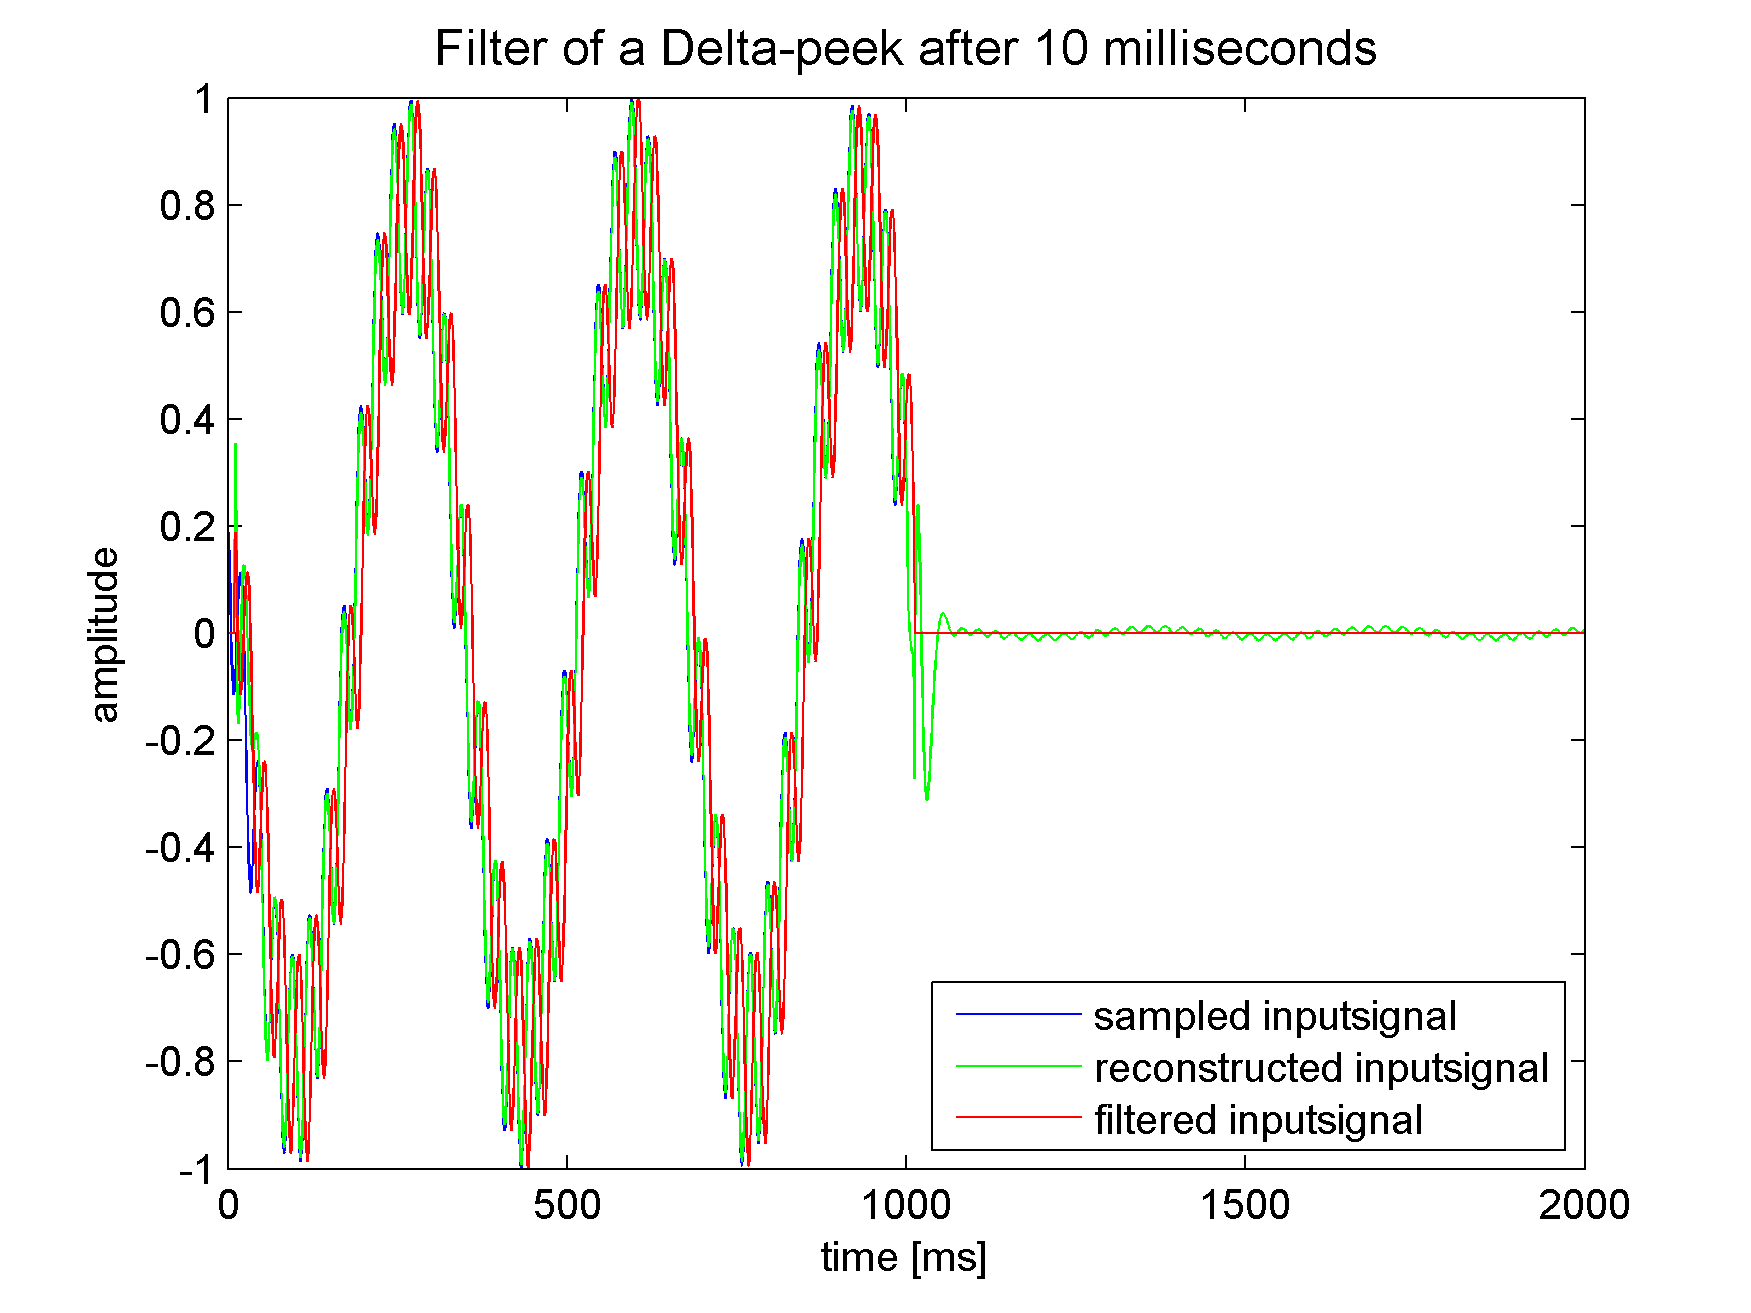
\includegraphics[width=0.6\textwidth]{afbeeldingen/plots/dp10ms.png}
        \end{subfigure}
        
        \begin{subfigure}[t]{\textwidth}
			    \caption{Used filter: a Delta-pulse at 500 ms, or 0.5 s}
			    \label{fig:app:test:toepl:05s}
                \centering
    			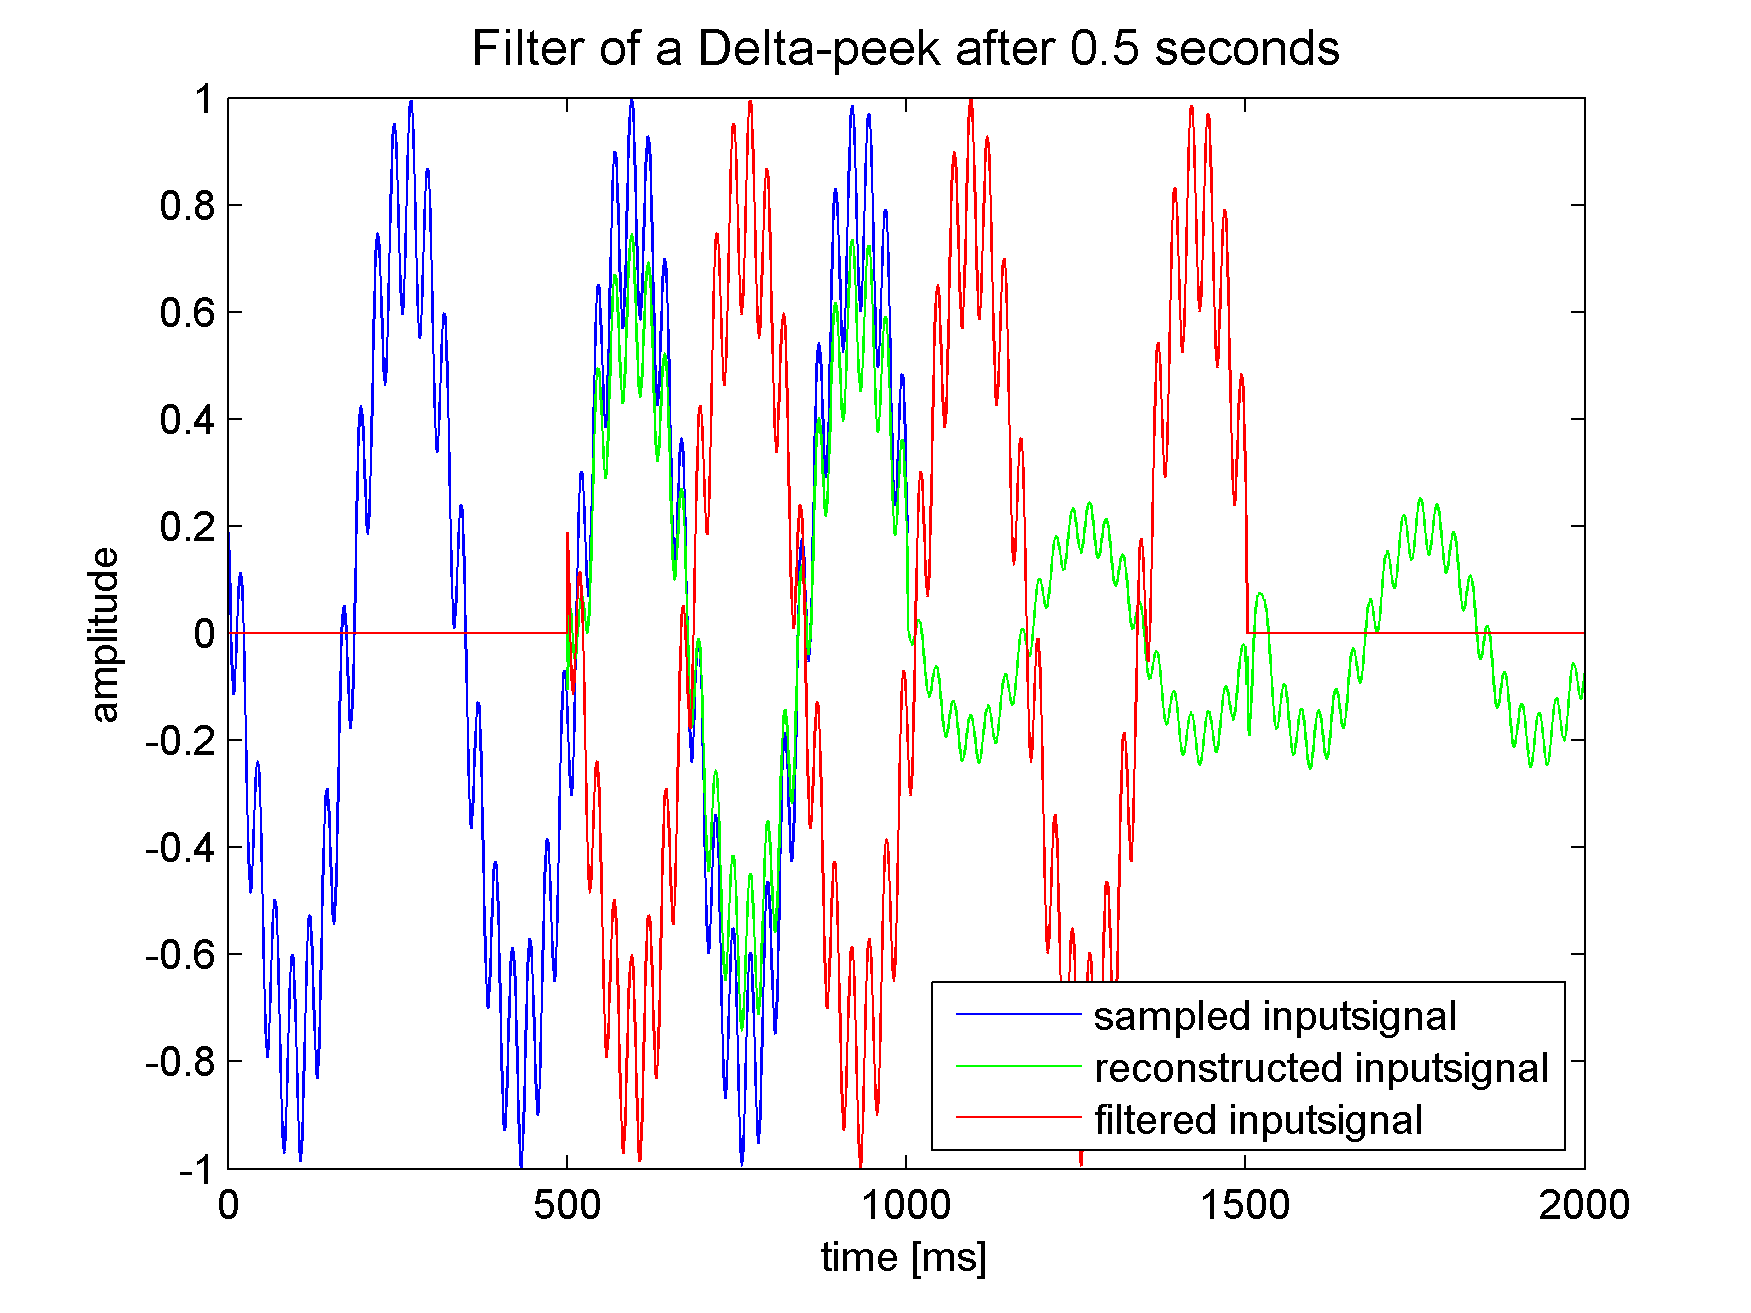
\includegraphics[width=0.6\textwidth]{afbeeldingen/plots/dp05s.png}
        \end{subfigure}
\end{figure}

\clearpage
\begin{figure}[h]
	    \caption[Results RLS method]{The results of finding a inverse filter using the RLS-method (described in Section \ref{ssec:rls}).\\
	    The test with simple input signals and filters worked very good, so here the results of the next step: the recorded signal (one TSP pulse) from the microphone. In \textbf{(a)} the response of the soundsystem has been caught in a FIR-filter with a length of 500 and the approximation has good results (the error is given by the red line), although a high forgetting factor is required.\\
	    In \textbf{(b)} the same has been tried for the inverse filter, with very poor result: a very high error between the estimation and the original system.}
	    \label{fig:app:test:rls}
        \centering
		\begin{subfigure}[t]{\textwidth}
			    \caption{Finding a FIR-filter for the soundsystem. Used RLS-settings: a filterlength of 500 and a forgetting factor of 0.999999.}
			    \label{fig:app:test:rls:soundsys}
                \centering
    			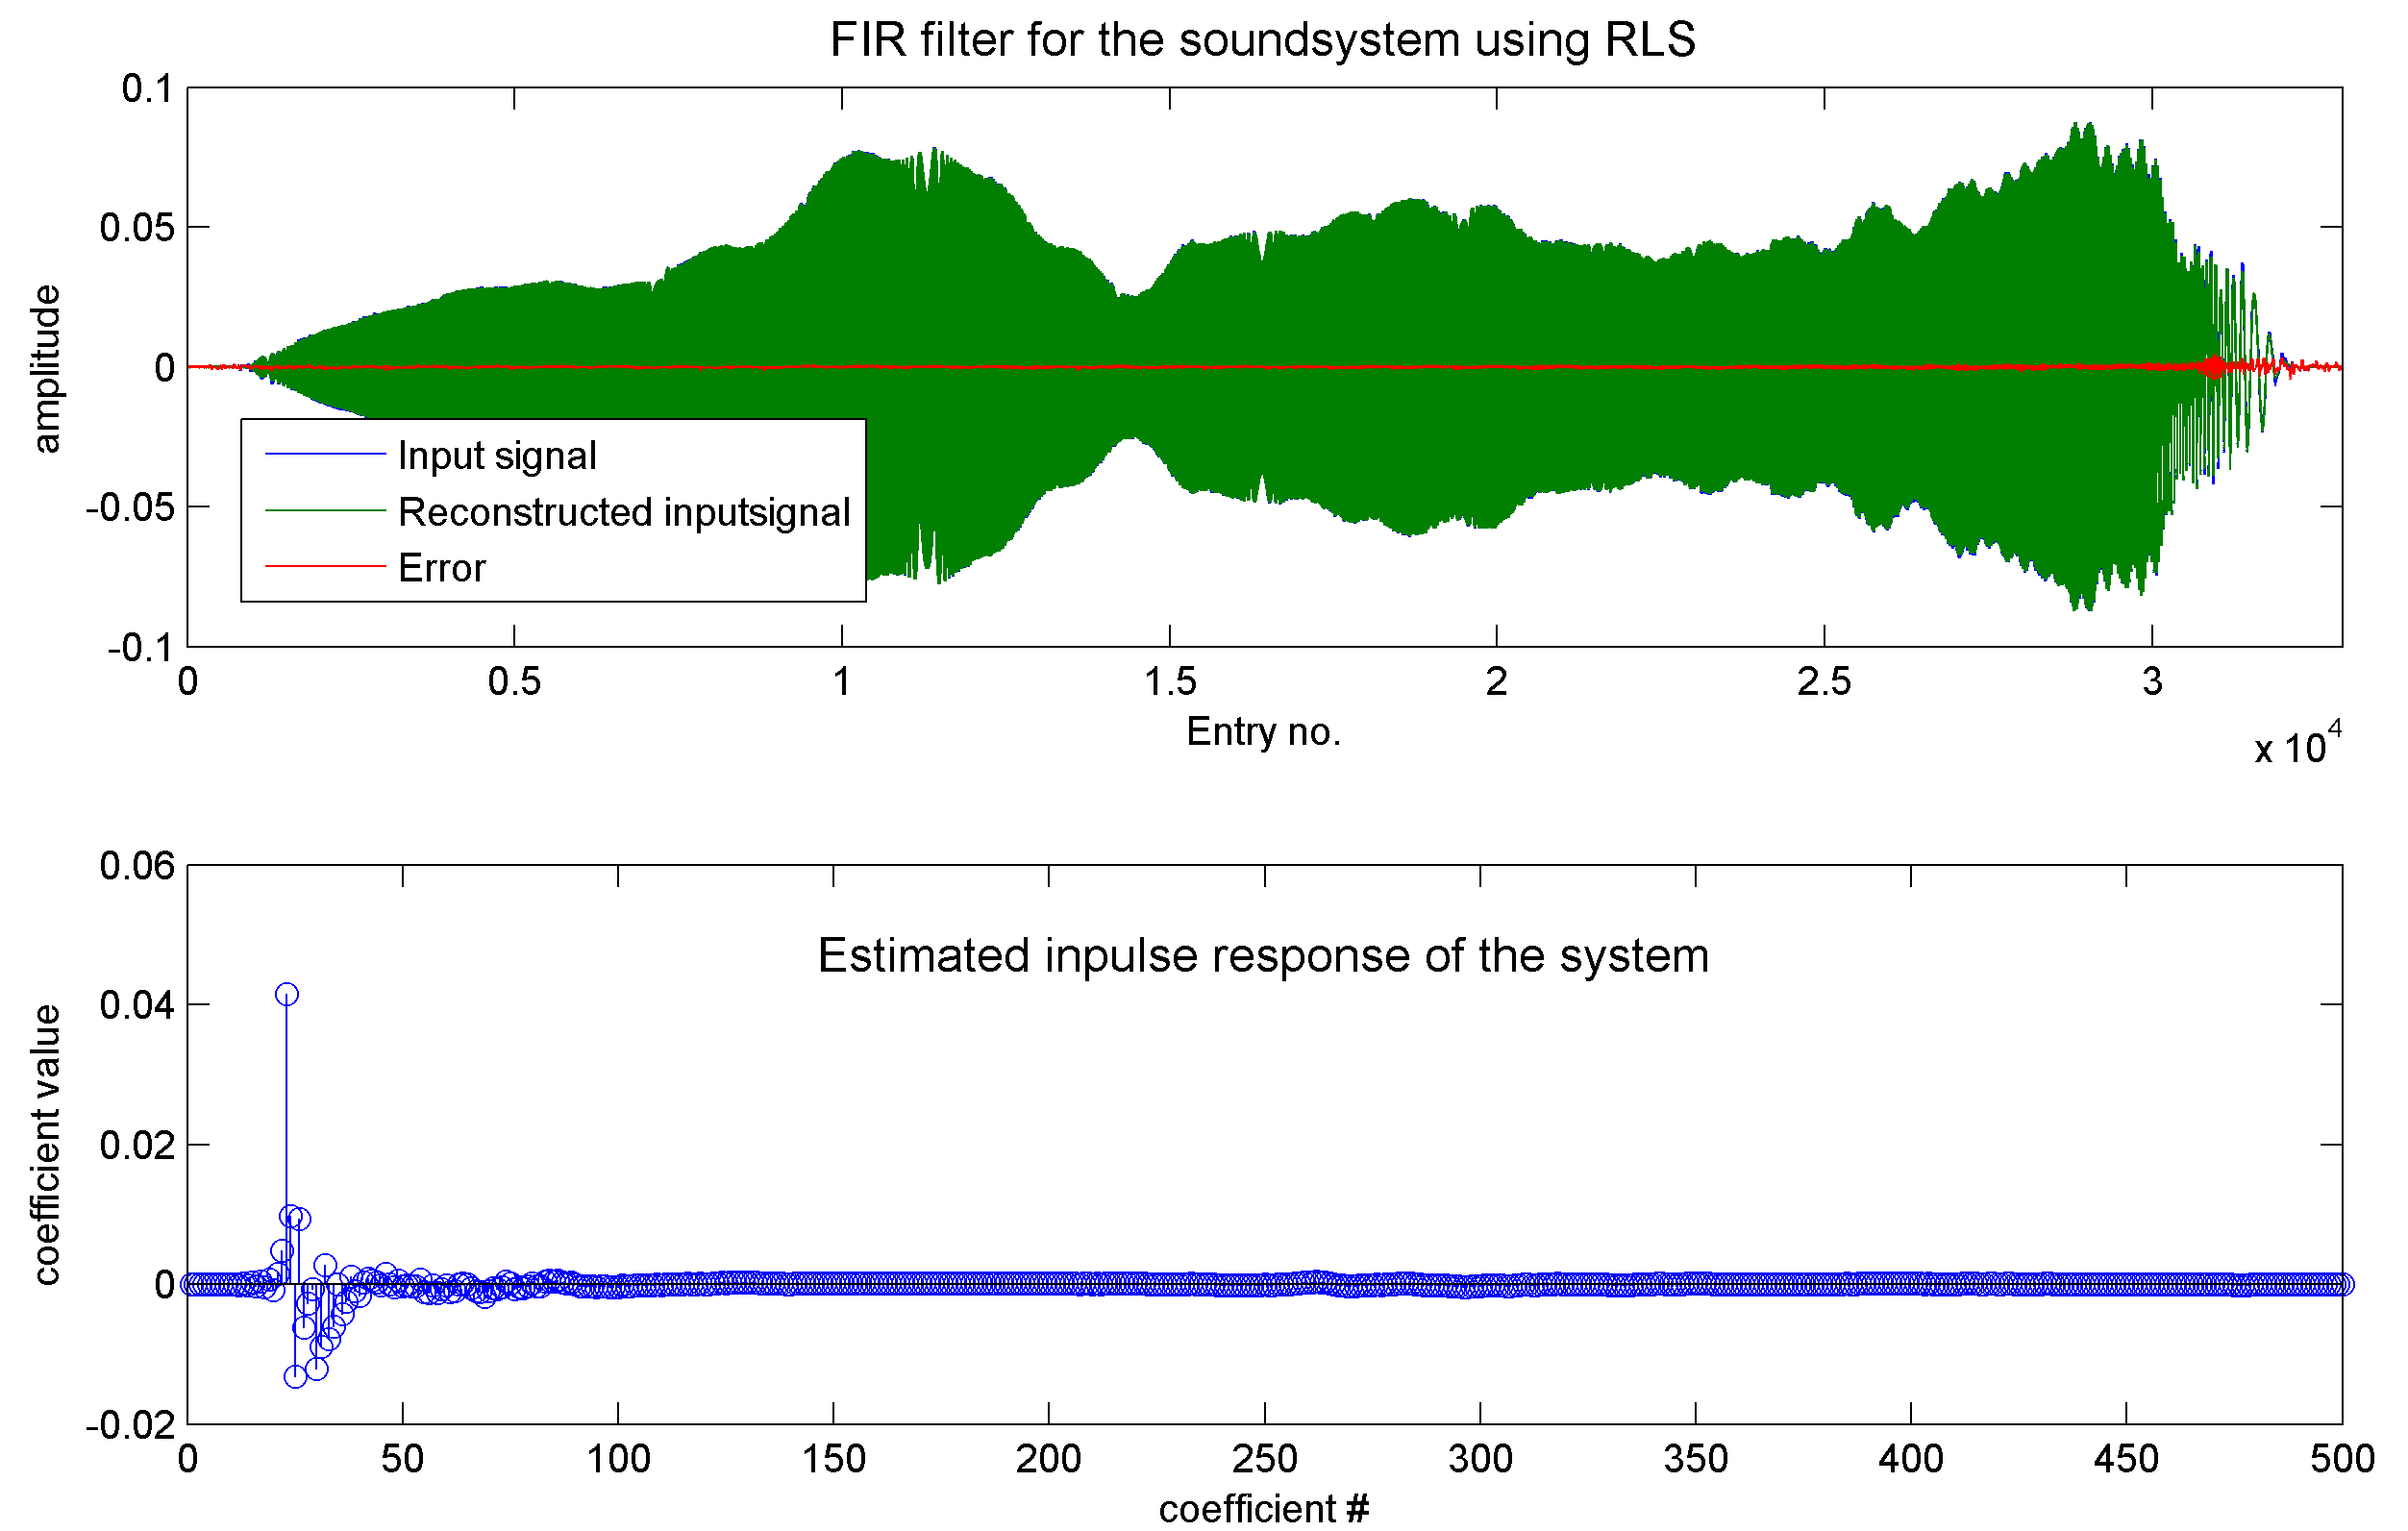
\includegraphics[width=\textwidth]{afbeeldingen/plots/filter_tspenkel_500_0999999_thesis.png}
        \end{subfigure}
        
        \begin{subfigure}[t]{\textwidth}
			    \caption{Finding a FIR-filter for the inverse of the soundsystem. Used RLS-settings: a filterlength of 500 and a forgetting factor of 0.999999. (Other settings did not have better results and took a lot of time to compute. Therefore the inverse filter with the same RLS-settings is shown.)}
			    \label{fig:app:rls:inv}
                \centering
    			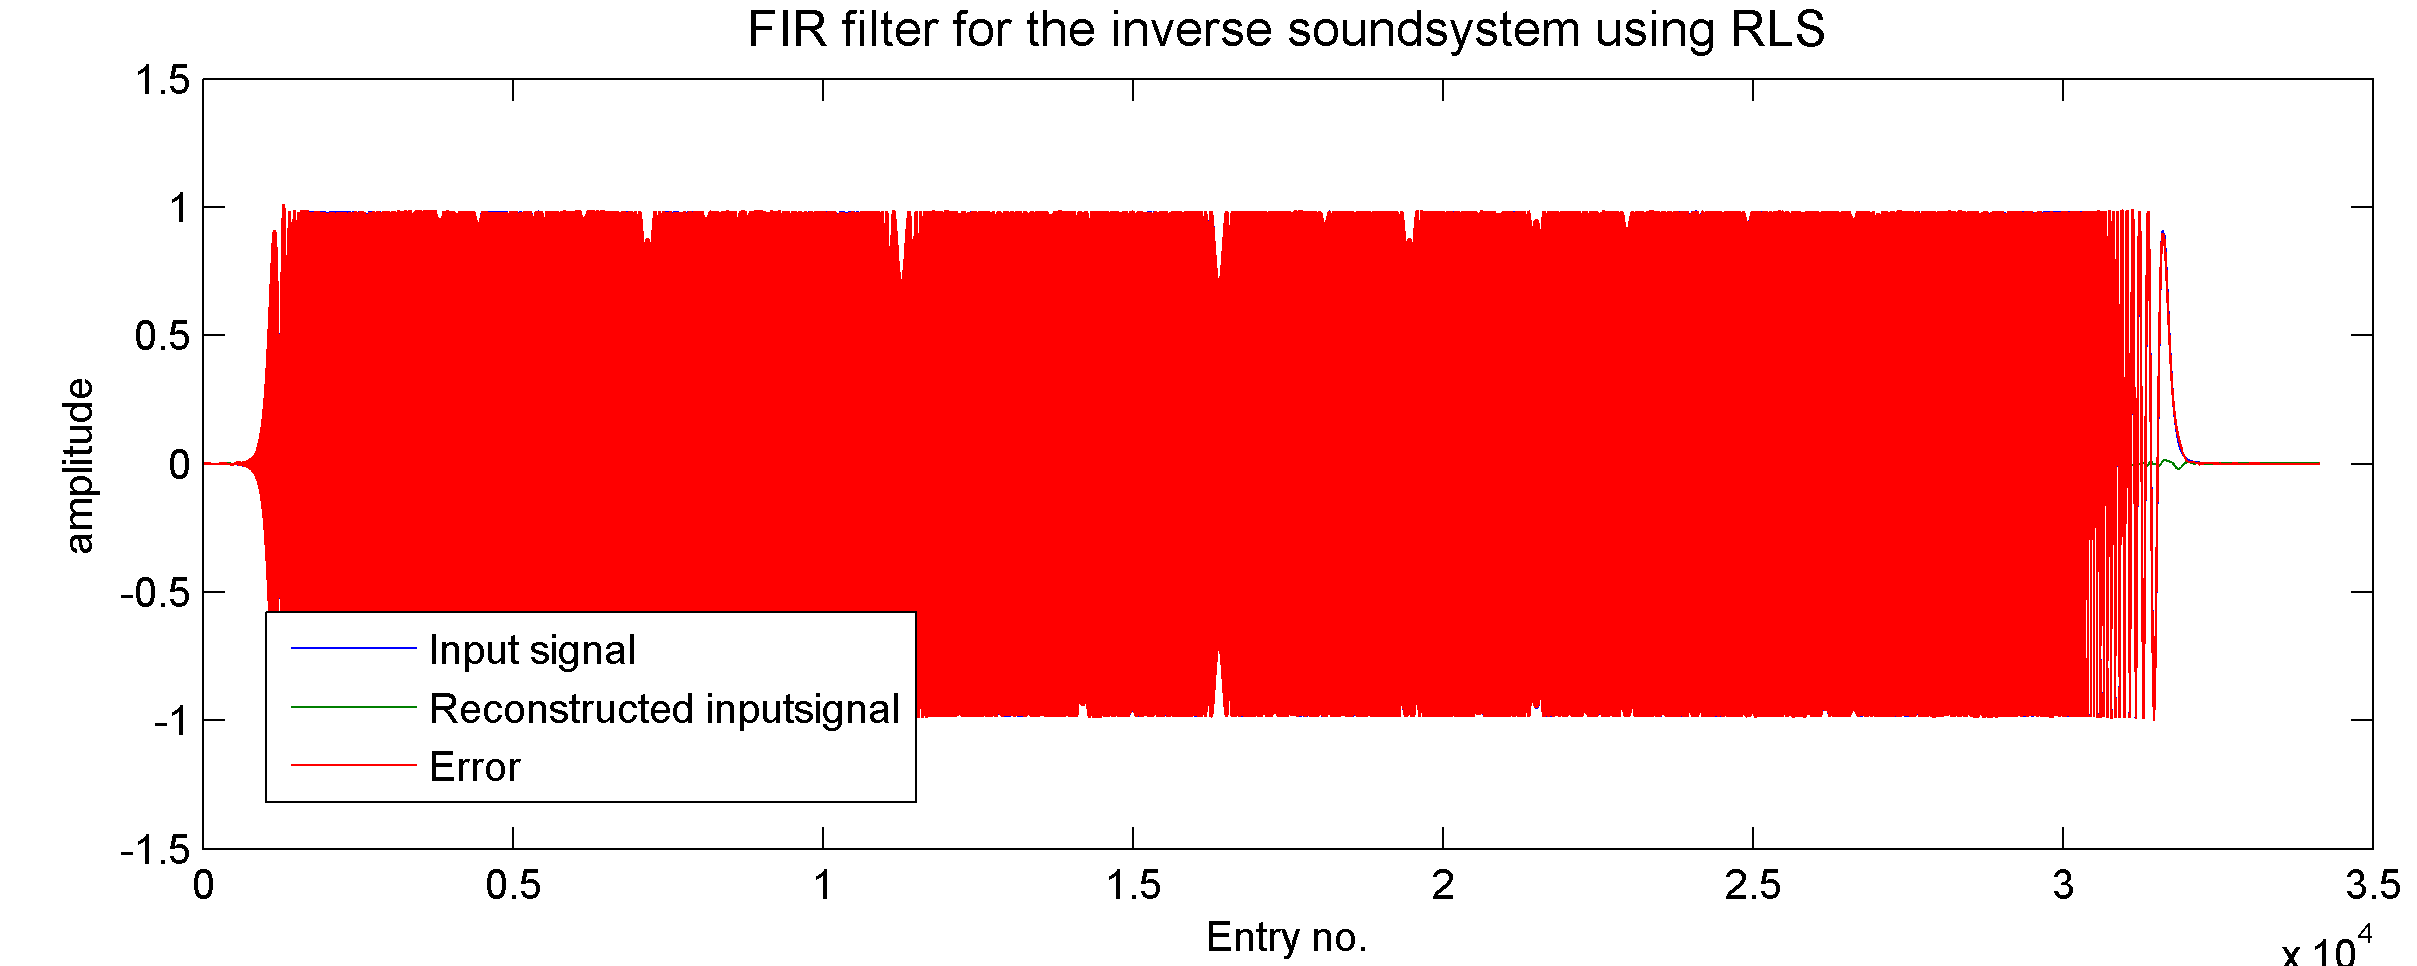
\includegraphics[width=\textwidth]{afbeeldingen/plots/invfilter_nocompute.png}
        \end{subfigure}
\end{figure}